\chapter{Introduction}\label{ch:intro}

\section{Variable stars}
Stars are called variable when there is a detectable change in brightness or color on time scales of the order
of the mean life time of humans~\cite{percy_2007, sterken_1996}.
The first claimed documented variable star is Algol visible with the unaided eye.
There exists ancient Egyptian calendars of lucky and unlucky days that possibly contain the periodicity of Algol\cite{porceddu_2008, porceddu_2018}.
The Cairo Calendar dated to 1244--1163 BC has been shown by Porceddu et al.~\cite{porceddu_2015} to represent Algol as Horus, a sky god and
symbol of kingship,
as seen in the figure~\ref{fig:horus} by matching the actions of Horus and the events witnessed by an observer of Algol.

\begin{figure}[h]
    \centering
    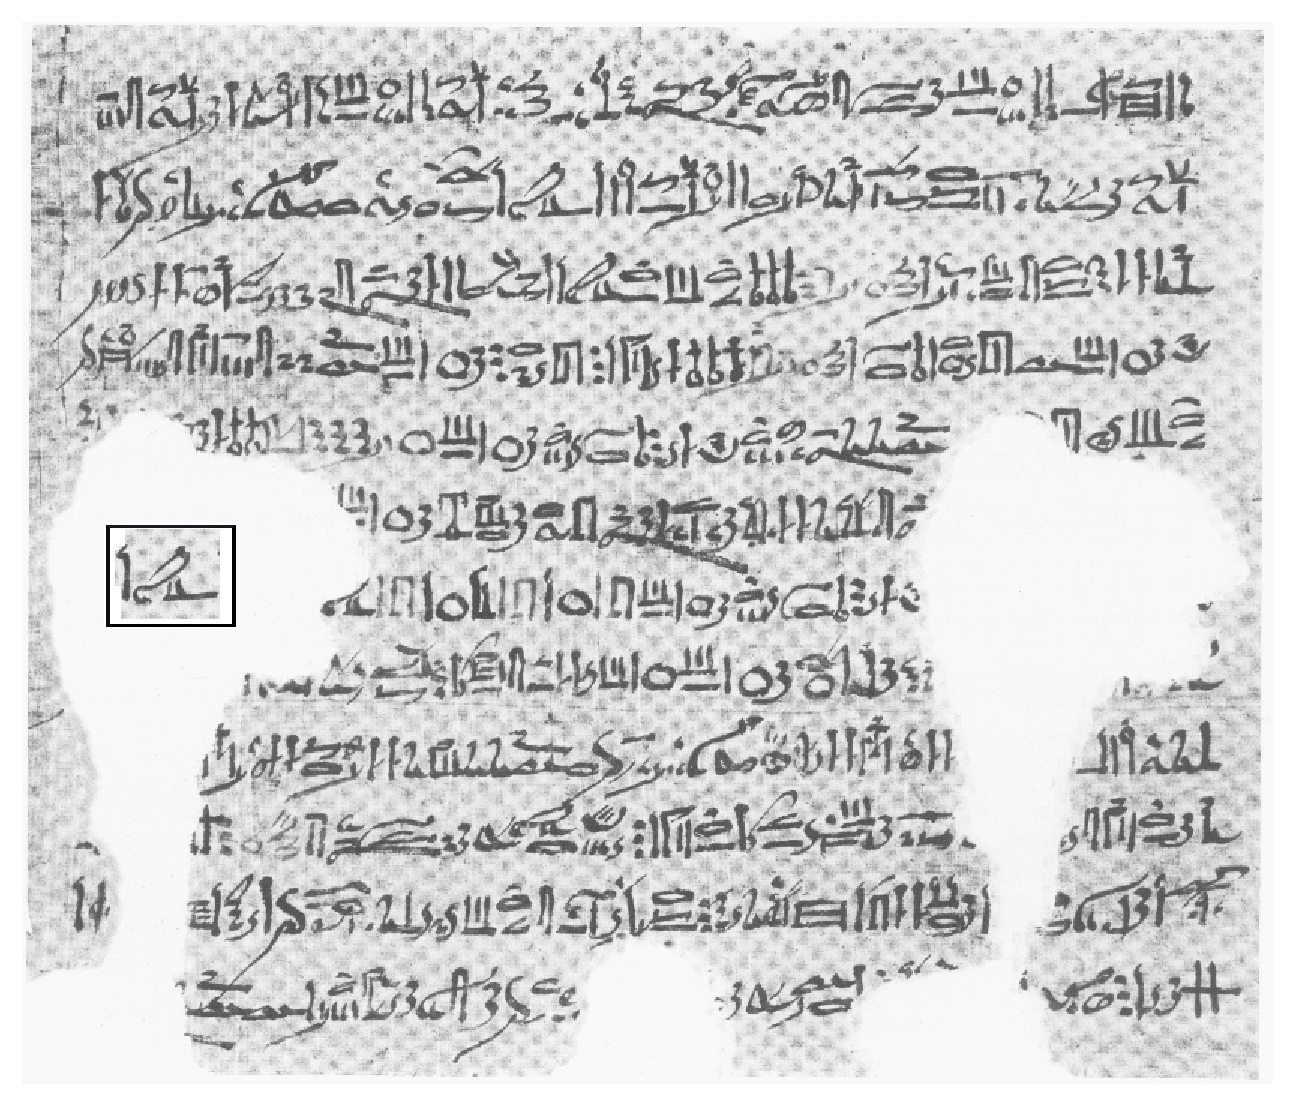
\includegraphics[width=\columnwidth]{figures/horus.eps}
    \caption{Inside the rectangle is the hieratic writing for the word Horus~\protect\cite{porceddu_2015}.}
\label{fig:horus}
\end{figure}

There is some curious relation between ancient Greek stories of the Gorgon Medusa, Perseus, the corresponding constellations, 
and the variable stars Algol and Omicron Ceti or more commonly named Mira (the wonderful).
Wilk~\cite{wilk_1996} suggests that the variability and location in the sky is embedded within the stories themselves.

The first recognized documented variable star, Omicron Ceti,  was recorded in 1596 and again in 1609 by David Fabricius while observing Jupiter.
Fabricius had first recorded Omicron Ceti as a nova, a singular event observed as a bright flash and quick dimming over the next few days,
comparing its significance with a supernova recorded by Tycho Brahe in 1572.
In 1638, Omicron Ceti was rediscovered by Johannes Phocylides Holwarda who found the periodic nature of this star to be approximately 11 months~\cite{hockey_2007}.

%In order to characterize eclipsing binary systems a light curve must be made.
%A light curve is a time series plot of the measured magnitude.

\section{Classifying variability}
Over time there have been several attempts to classify variable stars.
Classification systems reflect the current understanding of the mechanisms behind variability.
The earliest variable star observers like Goodricke and Pigott, who was employed to verify the variability of stars~\cite{pigott_1785}, would try to make sense of the observations and periods recorded by comparing and grouping different stars to those like Algol and $\omicron$ Ceti.  

One of the first attempts that went into detail was made by E.\ C.\ Pickering~\cite{sterken_1996, hoffleit_1972} in 1881 where he classified variable stars into the following categories\cite{pickering_1881}:
\begin{description}
    \item [Type I] Temporary stars. Examples, Tycho Brahe's star of 1572, new star in Corona, 1866.
    \item [Type II] Stars undergoing great variations in light in periods of several months or years. Examples, $\omicron$ Ceti and $\chi$ Cygni.
    \item [Type III] Stars undergoing slight changes according to laws yet unknown
    \item [Type IV] Stars whose light is continually varying, but the changes are repeated with great regularity in a period not exceeding a few days. 
    \item [Type V] Stars which every few days undergo for a few hours a remarkable diminution in light, this phenomenon recurring with great regularity. 
\end{description}

As time passes with more observations of variable stars, the collective understanding of the mechanisms of variability are improved.
With an improved understanding of physical processes including stellar evolution, pulsation, rotation, and eclipsing, then the taxonomy of classes is refined.

Since 1946, on behalf of the International Astronomical Union (IAU), Moscow variable star researchers have compiled detailed catalogs and certified 
variable stars in the General Catalogue of Variable Stars (GCVS). 
GCVS 5.1 is the most current version of the catalog containing $52,011$ variable objects discovered and named as variable stars by 2015~\cite{samus_2017}.

\subsection{General Catalogue of Variable Stars 5.1 Variability Types}
Variability types are in groups according to the major astrophysical reasons for variability.
The variable types have letter designations that typically corresponds to the original star that is observed with the same type of variability.
For example, in the eruptive group there is a type called GCAS that signifies eruptive irregular variables of the Gamma Cas type.
The definitions of the variable types are given by GVCS and maintained on their
website: \url{http://www.sai.msu.su/gcvs/gcvs/}

The following are groups with the variable types in those groups.
The reader can visit the GCVS Variability Types webpage\footnote{GCVS Variability Types: \url{http://www.sai.msu.su/gcvs/gcvs/vartype.htm}} to 
see specific variable types. 
\begin{description}
    \item [eruptive] FU, GCAS, I, IA, IB, IN, INA, INB, INT, IT, IN (YY), IS, ISA, ISB, RCB, RS, SDOR, UV, UVN, WR,
    \item [pulsating] ACYG, BCEP, BCEPS, CEP, CEP (B), CW, CWA, CWB, DCEP, DCEPS, DSCT, DSCTC, GDOR, L, LB, LC, M, PVTEL, RPHS, RR, RR (B), RRAB,
           RRC, RV, RVA, RVB, SR, SRA, SRB, SRC, SRD, SXPHE, ZZ, ZZA, ZZB,
    \item [rotating] ACV, ACVO, BY, ELL, FKCOM, PSR, SXARI,
    \item [cataclysmic (explosive and novalike) variables] N, NA, NB, NC, NL, NR, SN, SNI, SNII, UG, UGSS, UGSU, UGZ, ZAND,
    \item [eclipsing binary systems] E, EA, EB, EW, GS, PN, RS, WD, WR, AR, D, DM, DS, DW, K, KE, KW, SD,
    \item [intense variable X-ray sources] X, XB, XF, XI, XJ, XND, XNG, XP, XPR, XPRM, XM,
    \item [other symbols] BLLAC, CST, GAL, L:, QSO, S, *, +, $\colon$
    \item [the new variability types] ZZO, AM, R, BE, LBV, BLBOO, EP, SRS, LPB
\end{description}

This document will not cover all the different variable stars types. 
The study specifically will focus on EW type eclipsing binary systems.  

\section{Characterizing variability}
Using different algorithms one can distinguish the difference between the types of variable star system.

This demonstrates RR Lyrae
This demonstrates Eclipsing binaries

The relation between orbital mechanics and light curves

This demonstrates solar spots

Complex systems can involve a combination of these different systems.

\section{Eclipsing Binary Characterization}
Binary stars can reveal physical properties by examining the light curves.
Current models use a process called WD code.

In this thesis a modified WD code will be used from the Physics of Eclipsing Binaries (PHOEBE)

\section{O-C calculations}
Observed minus Calculated

\section{Equations of motion}

\section{WD code}
\subsection{Modified WD code}

\section{Pipeline for variable star detection}
\begin{enumerate}
    \item Data needs to be cleaned first.
    \item Align frames
    \item Extract sources
    \item Cross match sources with catalogs
    \item Create Database of known sources
    \item Plot individual light curves
    \item Analyze individual light curves for variability estimation
    \item Sort database given variability ranking
\end{enumerate}




\section{Data Acquisition}
Eclipsing binary optical data acquisition requires an observer to take time series ccd photometry of one target with an observation cadence dependent on the period.

A cadence can be determined by 

For example, the data gathered for this project was collected on multiple nights and observed on the order of hours with evenly timed frames.

\section{Known information of targets examined}

